\subsection{双轻子测量历史}

在历史上,许多实验都进行过双轻子的测量,并且得到了十分显著的成果,在这一小节中将会对历史上的双轻子测量进行一个简要的回顾。

\subsubsection{NA45实验}
环形切伦科夫电子能谱仪(Cherenkov Ring Electron Spectrometer, CERES, aka NA45),即NA45实验是位于欧洲核子中心(Conseil Européenn pour la Recherche Nucléaire, CERN)的超级质子同步加速器(Super Proton Synchrotron, SPS)上的能谱仪。其可以用两个对称的环状切伦科夫探测器来对电子进行鉴别从而测量双电子谱。NA45首先对p+Be和p+Au系统低质量区间的双电子谱进行了测量,结果如图 \ref{fig:NA45pA} 所示。可以看到进行了背景扣除的双电子谱可以被强子衰变模拟很好地描述。同时这两个测量表明强子衰变模拟可以很好的描述初始的冷核物质效应。

\begin{figure}[htb]
    \centering
    \begin{subfigure}[b]{0.47\textwidth}
        \centering
        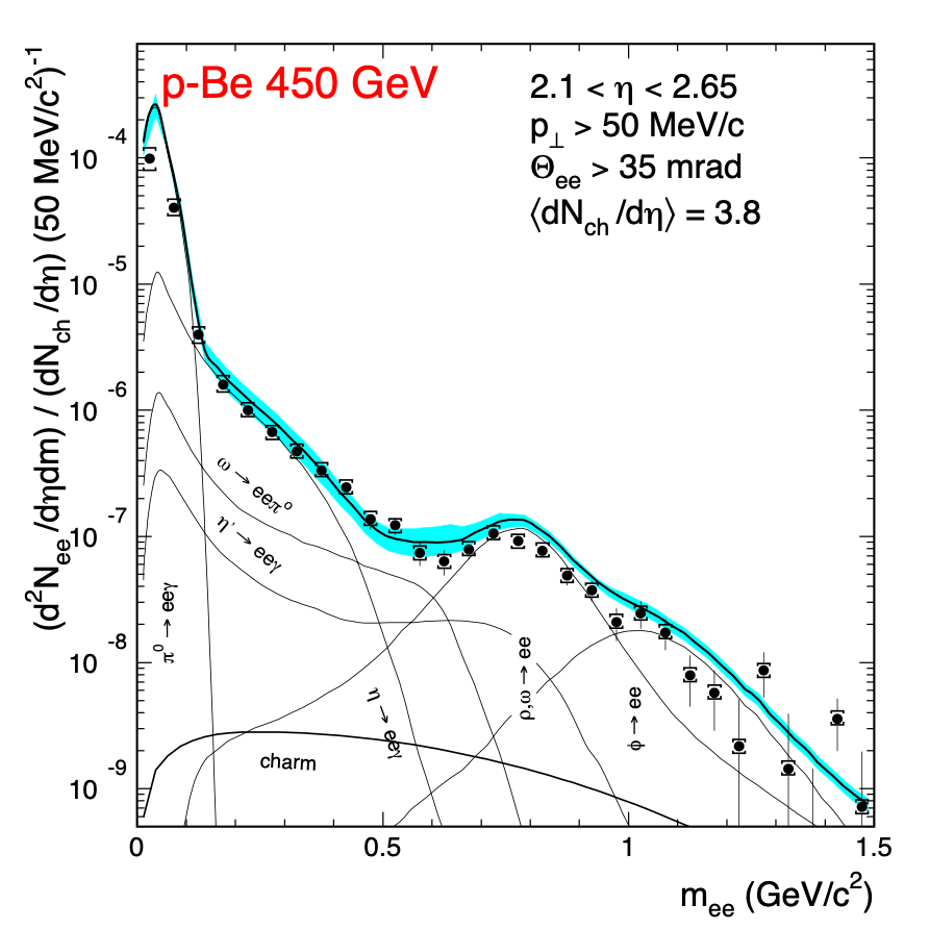
\includegraphics[width=\textwidth,clip]{figures/Chapter1/NA45pBe.png}
        \caption{}
        \label{fig:NA45pBe}
    \end{subfigure}
    \hfill
    \begin{subfigure}[b]{0.47\textwidth}
        \centering
        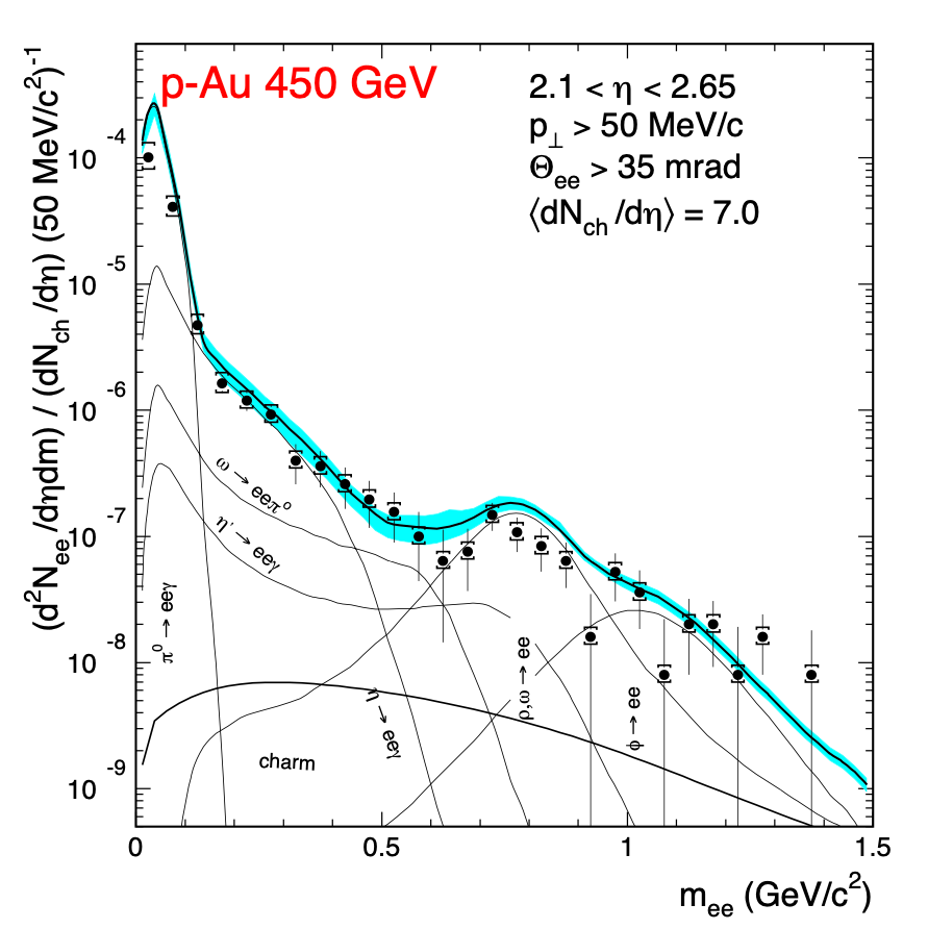
\includegraphics[width=\textwidth,clip]{figures/Chapter1/NA45pAu.png}
        \caption{}
        \label{fig:NA45pAu}
    \end{subfigure}
    \caption[NA45实验p+Be及p+Au对撞中低质量区间双电子谱]{NA45实验450 GeV p+Be \ref{fig:NA45pBe} 以及p+Au \ref{fig:NA45pAu} 对撞中的双电子谱。图中黑色实心圆点为数据点,黑线为强子衰变模拟结果。青色的error band代表了强子衰变模拟的系统误差。}
       \label{fig:NA45pA}
\end{figure}

之后NA45实验也对重离子对撞中的双电子谱进行了测量,图 \ref{fig:NA45SAu} 和图 \ref{fig:NA45PbAu} 分别展示了在200 AGeV 的硫-金对撞和 158 AGeV 铅-金对撞中的双电子谱。在这两个测量中可以看到数据点喝强子衰变模拟相比都有明显的额外产额增强。理论家们提出了一些模型来试图通过热辐射来解释这些额外产额,例如$\pi^+ + \pi^- \leftrightarrow \rho \rightarrow e^+ + e^-$过程。但当这些模型使用真空中的$\rho$质量谱的时候人们发现并不能很好的描述数据。这使得两种关于介质中的$\rho$不变质量谱的模型被提出来用以描述数据,分别是dorpping $\rho$ mass model 和 broadened $\rho$ model。这两种模型和数据的比较见图 \ref{fig:NA45PbAu}。但受限于统计,NA45的结果无法对这两种模型是否能很好的描述数据进行有效的分辨。这两种模型的比较直到后来NA60的更高精度双 \muon 谱测量结果出炉后才有了一个相对明确的结论。

\begin{figure}[htb]
    \centering
    \begin{subfigure}[b]{0.47\textwidth}
        \centering
        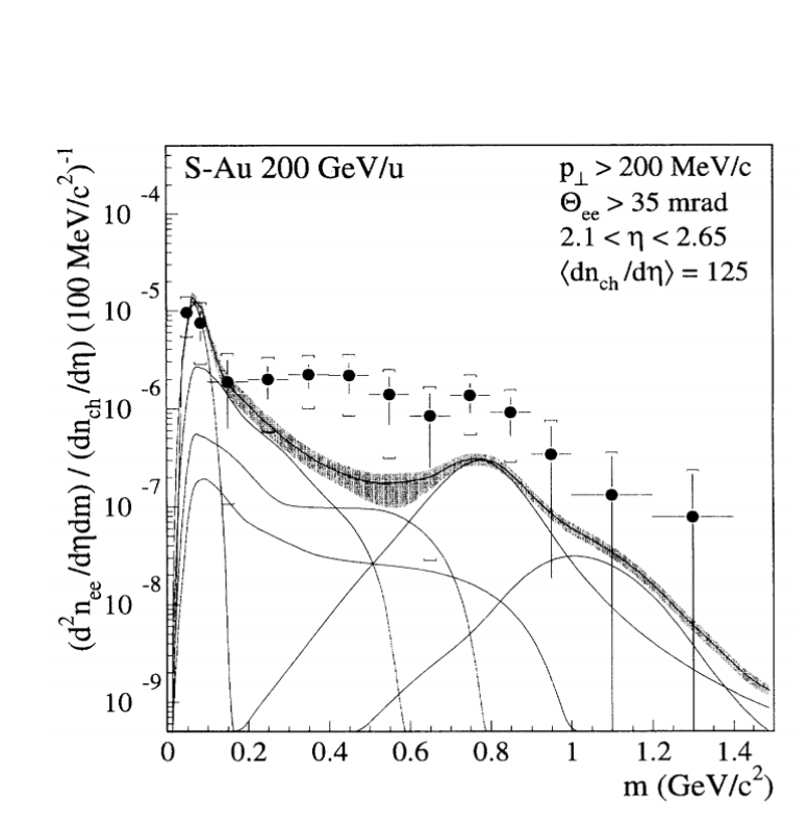
\includegraphics[width=\textwidth,clip]{figures/Chapter1/NA45SAu.png}
        \caption{}
        \label{fig:NA45SAu}
    \end{subfigure}
    \hfill
    \begin{subfigure}[b]{0.47\textwidth}
        \centering
        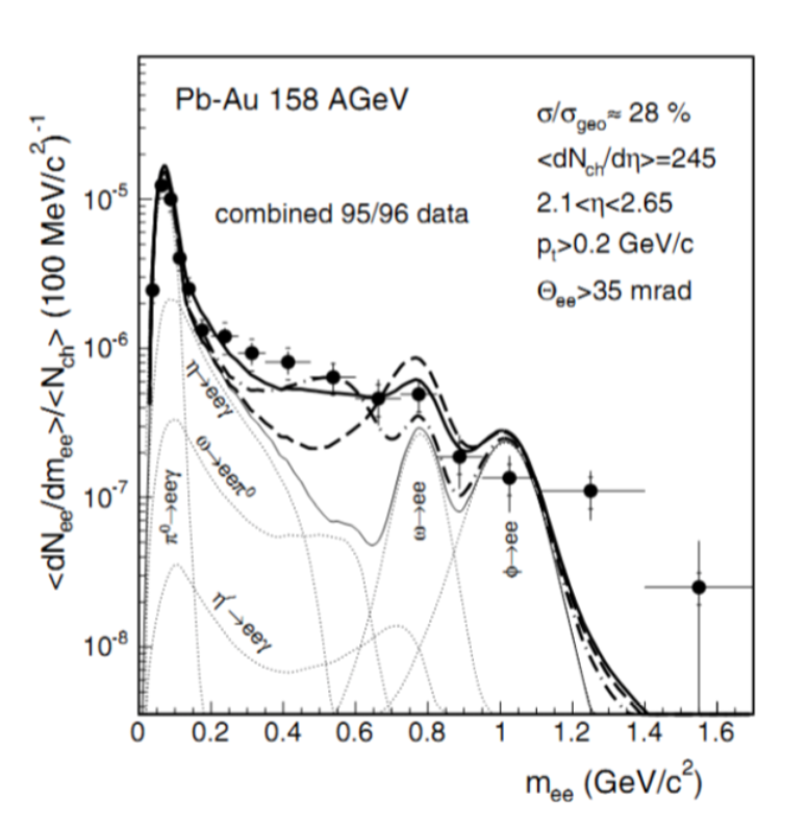
\includegraphics[width=\textwidth,clip]{figures/Chapter1/NA45PbAu.png}
        \caption{}
        \label{fig:NA45PbAu}
    \end{subfigure}
    \caption[NA45实验200 AGeV 硫-金及 158 AGeV 铅-金对撞中的双电子谱]{NA45实验中测得的200 AGev 硫-金对撞中的双电子谱\ref{fig:NA45SAu}和158 AGeV 铅-金对撞中的双电子谱\ref{fig:NA45PbAu}。右图中虚线为强子衰变模拟+真空中$\rho$双电子谱的模拟结果。两种不同的描述$\rho$的不变质量谱变化的模型一并被放入了图中,分别为在图中以点划线表示的dorpping $\rho$ mass model和以粗实线表示的broadened $\rho$ model。}
       \label{fig:NA45AA}
\end{figure}

\subsubsection{NA60实验}

NA60实验为超级质子同步加速器上的固定靶实验。因为NA60实验所拥有的高精度的 \muon 谱仪和顶点探测器,使得其有能力进行高质量分辨(~20 $\rm{MeV/c^20}$)和高位置分辨($ \sigma_x < 10 \mu m$,$\sigma_x < 15 \mu m$)的测量。基于高精度的实验设置,NA60可以有效的去除来自于弱衰变(例如 $\pi^{\pm} \rightarrow \mu^{\pm} + \nu_{\mu}(\bar{\nu}_{\mu})$和$K^{\pm} \rightarrow \mu^{\pm} + \nu_{\mu}(\bar{\nu}_{\mu})$)的背景和来源于重味半轻子衰变的 \muon 。NA60对 \sNN = 17.3 GeV 铟-铟对撞中的双 \muon 谱进行了测量,在全部中心度区间和“半中心”(semicentral)中心度区间的测量结果分别如图 \ref{fig:NA60NoCen} 和 \ref{fig:NA60SemiCentral}所示。
在“半中心”对撞的测量结果在扣除强子衰变模拟(不含 $\rho$)后和不同理论模型预测的$\rho$的不变质量谱进行了比较,因为该测量有着很高的精度,结果可以对理论模型的结果进行很好的约束。可以看到dropping $\rho$ 模型并不能描述数据而 broaden $\rho$ 模型可以在 $0.2 <  M_{\mu\mu} < 0.8~{\rm GeV/c^2} $的质量区间里很好的描述数据。
\begin{figure}[htb]
    \centering
    \begin{subfigure}[b]{0.47\textwidth}
        \centering
        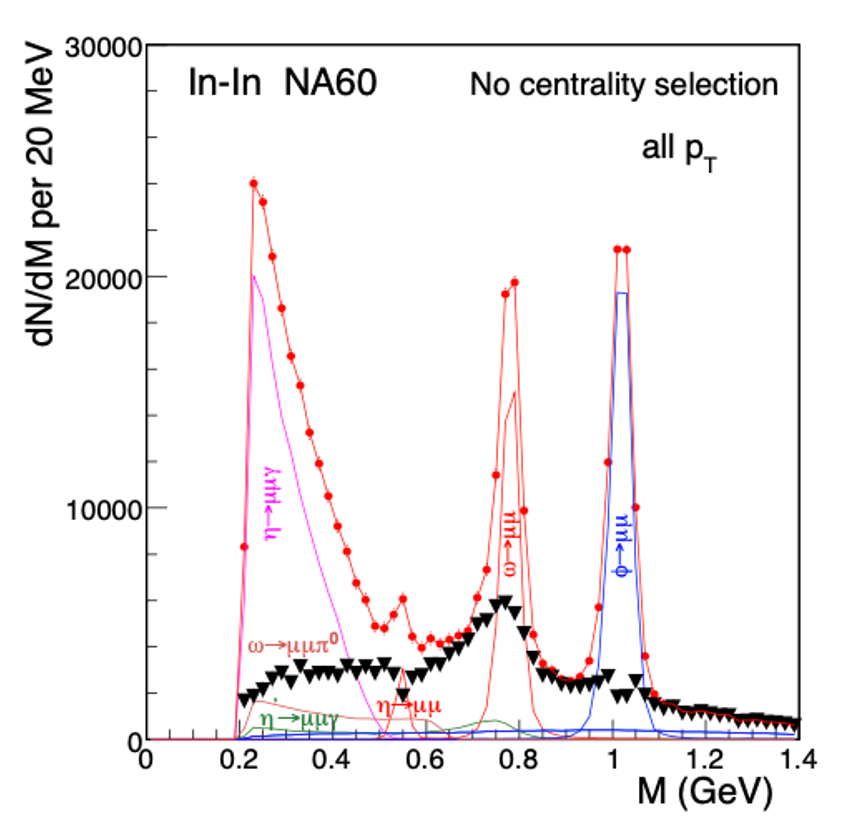
\includegraphics[width=\textwidth,clip]{figures/Chapter1/NA60NoCen.png}
        \caption{}
        \label{fig:NA60NoCen}
    \end{subfigure}
    \hfill
    \begin{subfigure}[b]{0.47\textwidth}
        \centering
        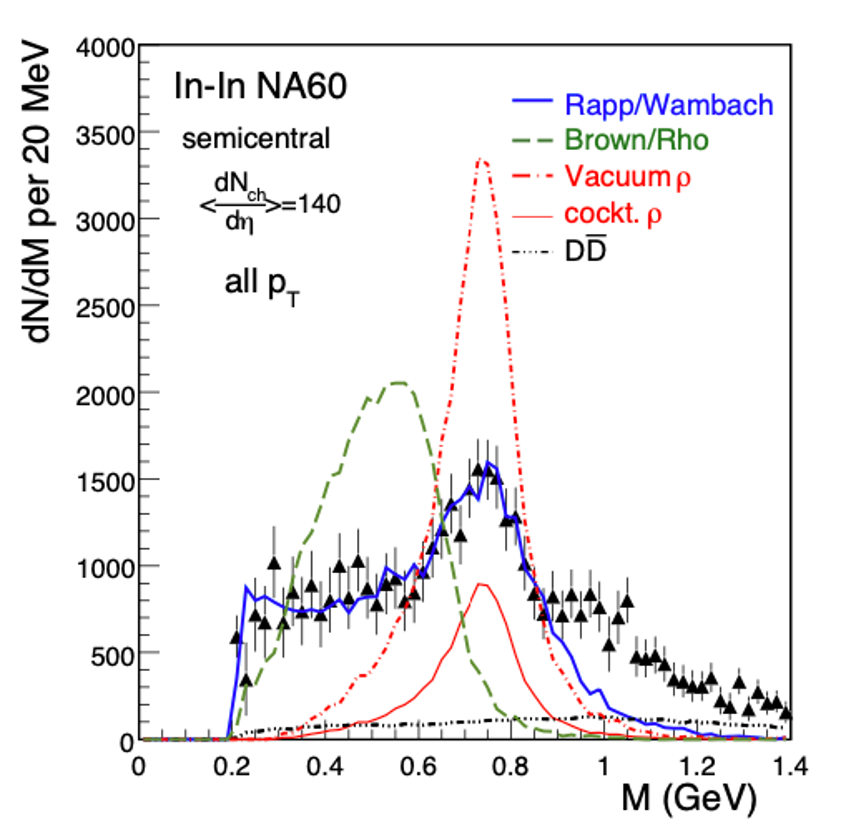
\includegraphics[width=\textwidth,clip]{figures/Chapter1/NA60SemiCentral.png}
        \caption{}
        \label{fig:NA60SemiCentral}
    \end{subfigure}
    \caption[NA60实验\sNN = 17.3 GeV 铟-铟对撞中的双 \muon 谱]{NA60实验\sNN = 17.3 GeV 铟-铟对撞中的双 \muon 谱。左图中未进行中心度筛选的双 \muon 谱,其中红色圆点为未扣除强子衰变模拟的双 \muon 谱,黑色三角为扣除强子衰变模拟后的双 \muon 谱。右图为扣除强子衰变模拟后在“半中心”中心度下的双 \muon 谱。来自不同模型预测的 $\rho$ 的产额在途中以不同形式的线标出。}
       \label{fig:NA60DiMuon}
\end{figure}

在更高的质量区间($M_{\mu\mu} > 0.8~{\rm GeV/c^2}$),双 \muon 的额外产额并不能被任何一种有关 $\rho$ 不变质量谱在介质中的修正模型来描述。在高精度的顶点测量探测器的帮助下NA60实验可以对双轻子的额外产额来源进行分析。经过分析,重味夸克的半轻子衰变和Drell-Yan过程被认为不是额外产额的主要来源。因为统计量足够,NA60进一步对不同的质量区间进行了$m_{T}~(m_{T} = \sqrt{p_T^2 + m^2})$谱的研究。在不同的质量区间用一个指数分布来拟合$m_T$谱,拟合方程为:$1/m_{T}*dN/dm_{T} \propto exp(-m_{T}/T_{eff})$。其中的反斜率参数$T_{eff}$可以被解释为介质的有效温度。在不同质量区间中的有效温度的拟合如图 \ref{fig:NA60T}所示。$T_{eff}$在大约1 GeV处的突然降低表明用强子产生并不能很好的解释在中等质量区间的双轻子额外产额,更自然的解释是这部分额外产额来源于介质的热辐射。

\begin{figure}[htb]
    \begin{center}
    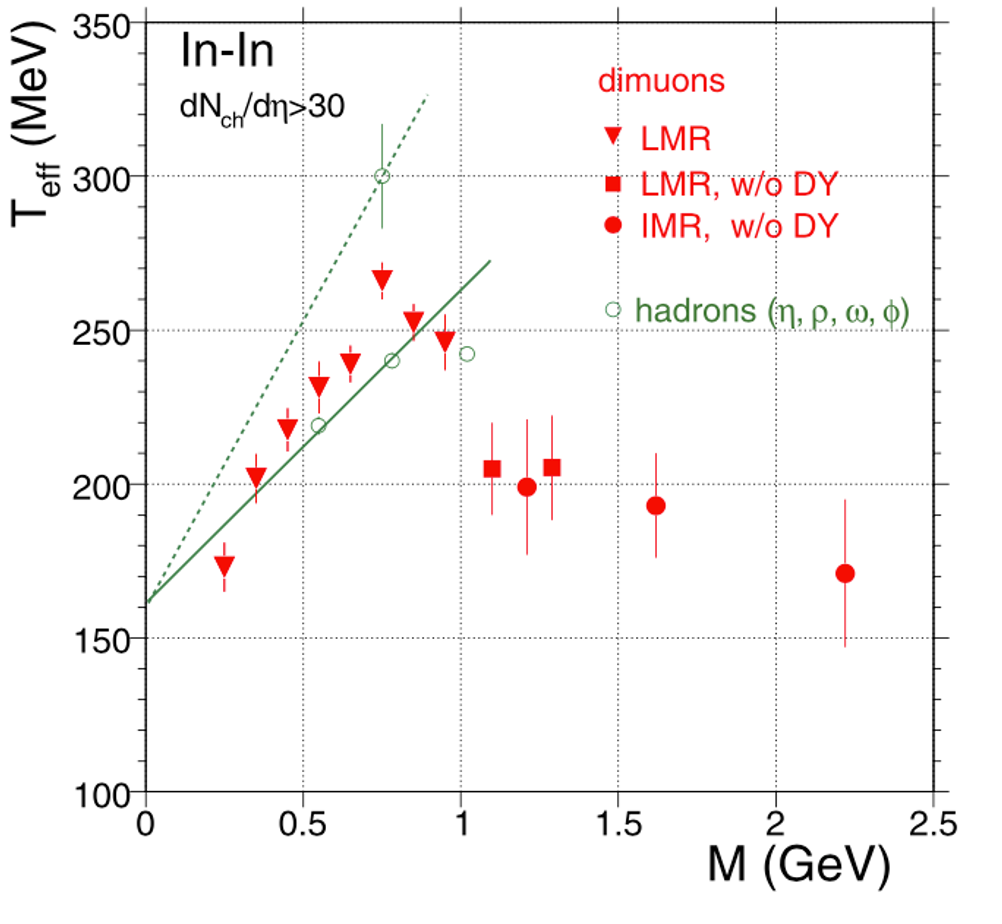
\includegraphics[width=0.75\textwidth,clip]{figures/Chapter1/NA60T.png}
    \end{center}
    \caption[NA60不同质量区间的有效温度测量结果]{NA60实验在不同质量区间下用$exp(-m_{T}/T_{eff})$拟合$m_T$谱得到的有效温度参数结果,并且与从强子谱得到的结果(绿色空心点)进行比较}
    \label{fig:NA60T}
\end{figure}

\subsubsection{PHENIX实验}

在RHIC上的双轻子测量主要由PHENIX(The Pioneering High Energy Nuclear Interaction eXperiment, PHENIX)实验和STAR(Solenoidal Tracker at RHIC)实验完成。

首先我们对PHENIX实验的双轻子测量结果进行一个简要的回顾。PHENIX实验是RHIC的两个大型粒子物理实验之一,其可以对中等快度区间内一定方位角的粒子进行测量,其探测器设计参数见参考文献[]。PHENIX首先对\sNN = 200 GeV质子-质子对撞中的双电子谱进行了测量,结果如图 \ref{fig:PHENIXpp} 所示。数据和强子衰变模拟的数据在误差范围内符合的很好,证明质子-质子对撞可以作为我们研究金-金对撞中的双电子谱时的基线。随后PHENIX也对 \sNN = 200 GeV 金-金对撞中的双电子谱进行了测量。在不同中心度下的结果如图 \ref{fig:PHENIXAuAu} 所示。在相对中心的对撞中心度下均观察到了在低质量区间($ 0.15 < M_{ee} < 0.75~{\rm GeV/c^2}$)相比于强子衰变模拟的产额增强。从图中也可以看到随着对撞接近中心对撞,这种产额增强的程度越来越高。这种增强和之前的预期相符。同时在低质量区间($M_{ee} < 0.3~{\rm GeV/c^2}$)和相对较高的横动量区间($ 1 < p_T < 5 ~{\rm GeV/c^2}$)的区间在质子-质子和金-金对撞中都观测到了产额的增强,在这个区间内的额外产额和质量的依赖关系和直生虚光子的产生的预测相符合。PHENIX也对直生虚光子进行了测量,但在本文中不进行详细的讨论,可参见参考文献[]。

\begin{figure}[htb]
    \centering
    \begin{subfigure}[b]{0.45\textwidth}
        \centering
        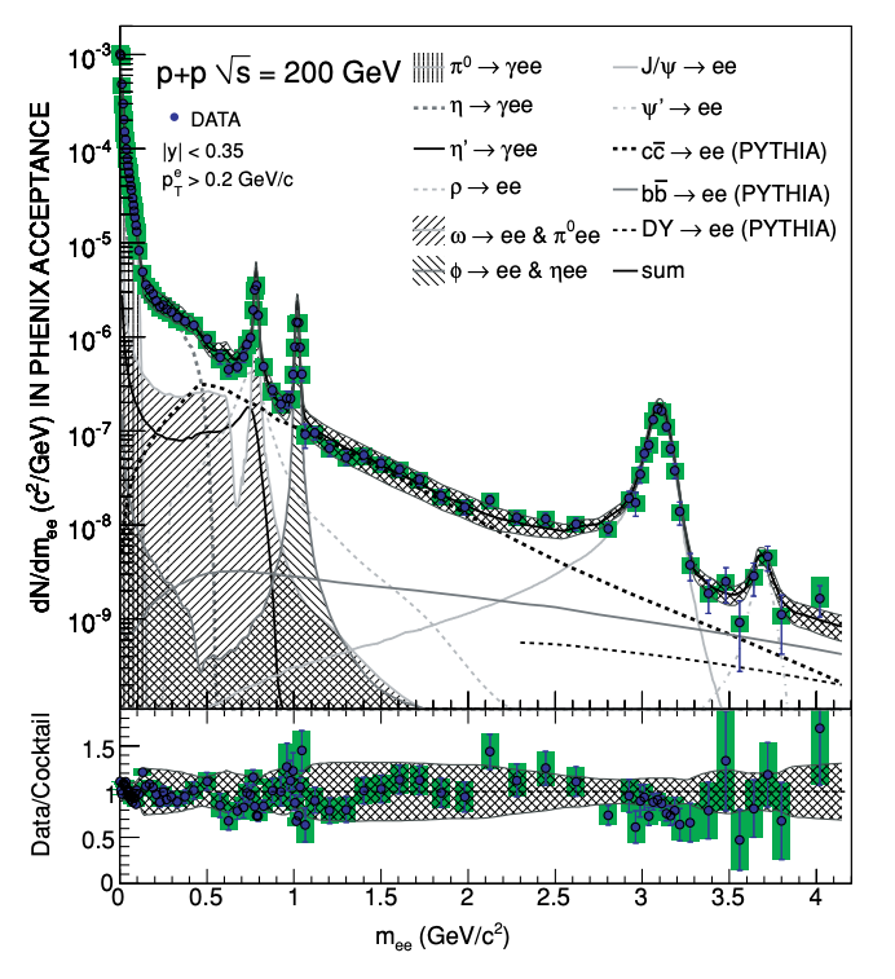
\includegraphics[width=\textwidth,clip]{figures/Chapter1/PHENIXpp.png}
        \caption{}
        \label{fig:PHENIXpp}
    \end{subfigure}
    \hfill
    \begin{subfigure}[b]{0.45\textwidth}
        \centering
        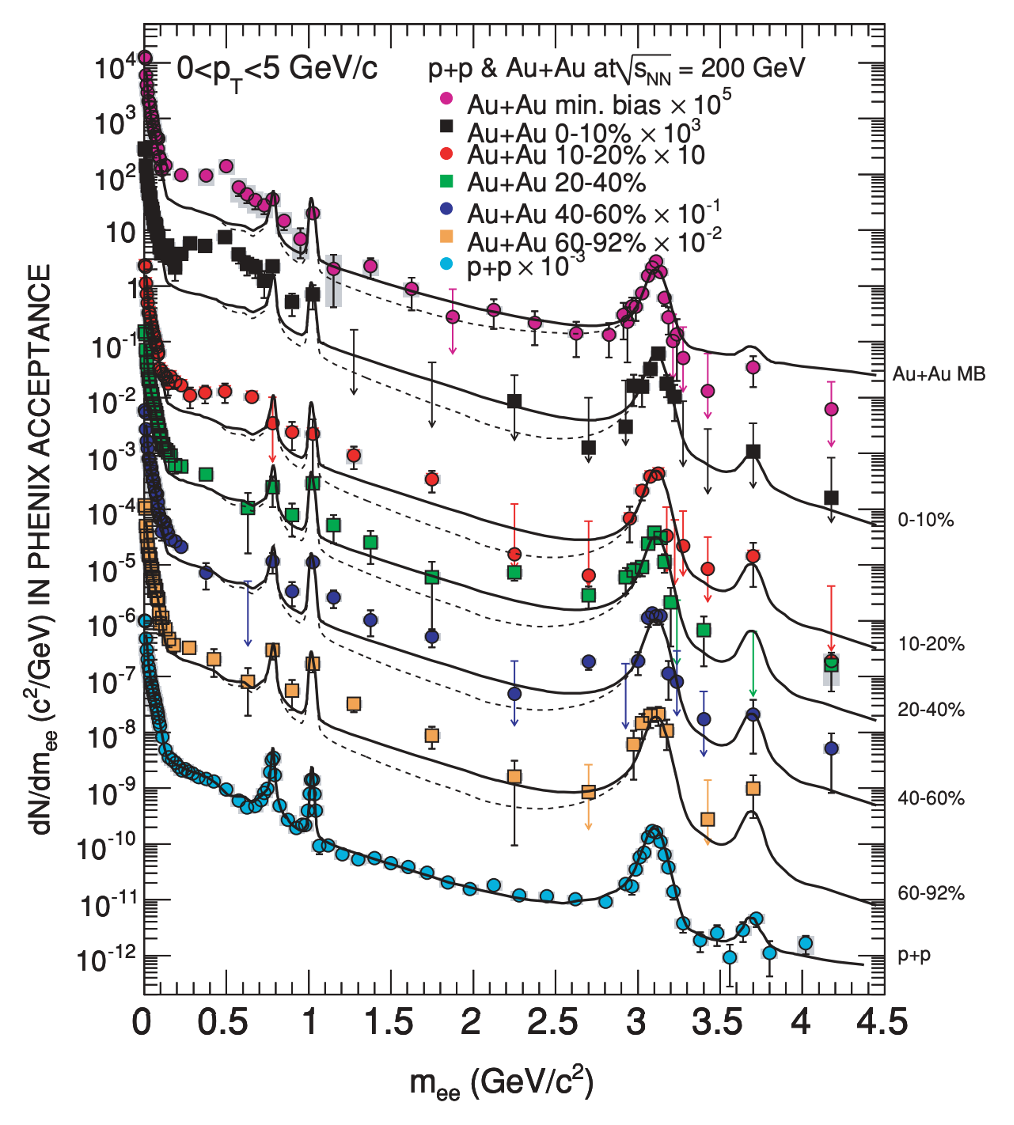
\includegraphics[width=\textwidth,clip]{figures/Chapter1/PHENIXAuAu.png}
        \caption{}
        \label{fig:PHENIXAuAu}
    \end{subfigure}
    \caption[PHENIX实验 \sNN = 200 GeV 质子-质子和金-金对撞中的双电子谱测量结果]{PHENIX实验在其接收度下的 \sNN = 200 GeV 质子-质子和金-金对撞中的双电子谱测量结果。左图为质子-质子对撞中的双电子谱测量结果。测量结果与强子衰变模拟的结果进行比较,强子衰变模拟的不同双电子源在图中已经标出。右图为\sNN = 200 GeV质子-质子和金-金对撞中不同中心度下的双电子谱。}
       \label{fig:PHENIXDiElectron}
\end{figure}

\subsubsection{STAR实验}

作为RHIC上的另一个大型粒子物理实验,STAR实验也对不同对撞系统和不同对撞能量中的双轻子谱进行了测量。在STAR的主径迹探测器时间投影室(Time Projection Chamber, TPC)和飞行时间探测系统(Time of Flight, TOF)的帮助下,STAR有能力获得高电子纯度的数据样本。以金-金 \sNN = 200 GeV 对撞的数据为例,其可获得电子纯度最高为94.6 ± 2 \%的数据样本。

和PHEINX实验类似,为了给离子-离子对撞中的测量定下一条好的基线,STAR的双轻子测量也是从质子-质子对撞开始的。STAR的首个双轻子测量结果基于2009年采集的质子-质子对撞数据,结果如图 \ref{fig:STARpp}所示。和PHENIX饰演的结果类似,强子衰变模拟也可以很好的描述测量到的双轻子谱。其中源自c夸克双电子模拟结果由PYTHIA6模拟得到。之后STAR合并2010和2011年两年的金-金 \sNN = 200 GeV下的数据进行了双电子谱的测量,如图 \ref{fig:STARAuAu}所示。在 $\rho$ 的质量区间($0.3 < M_{ee} < 0.76 ~{\rm GeV/c^2}$)STAR观测到了相比于强子衰变模拟1.76 ± 0.06 (stat) ± 0.26 (systematic) ± 0.29 (cocktail)倍的产额增强。STAR在 \sNNerbai 金金对撞中的测量结果在统计误差范围内和PHENIX合作组的测量结果可以符合,并且对于额外产额也和几种不同的理论模型进行了比较。

\begin{figure}[htb]
    \centering
    \begin{subfigure}[b]{0.43\textwidth}
        \centering
        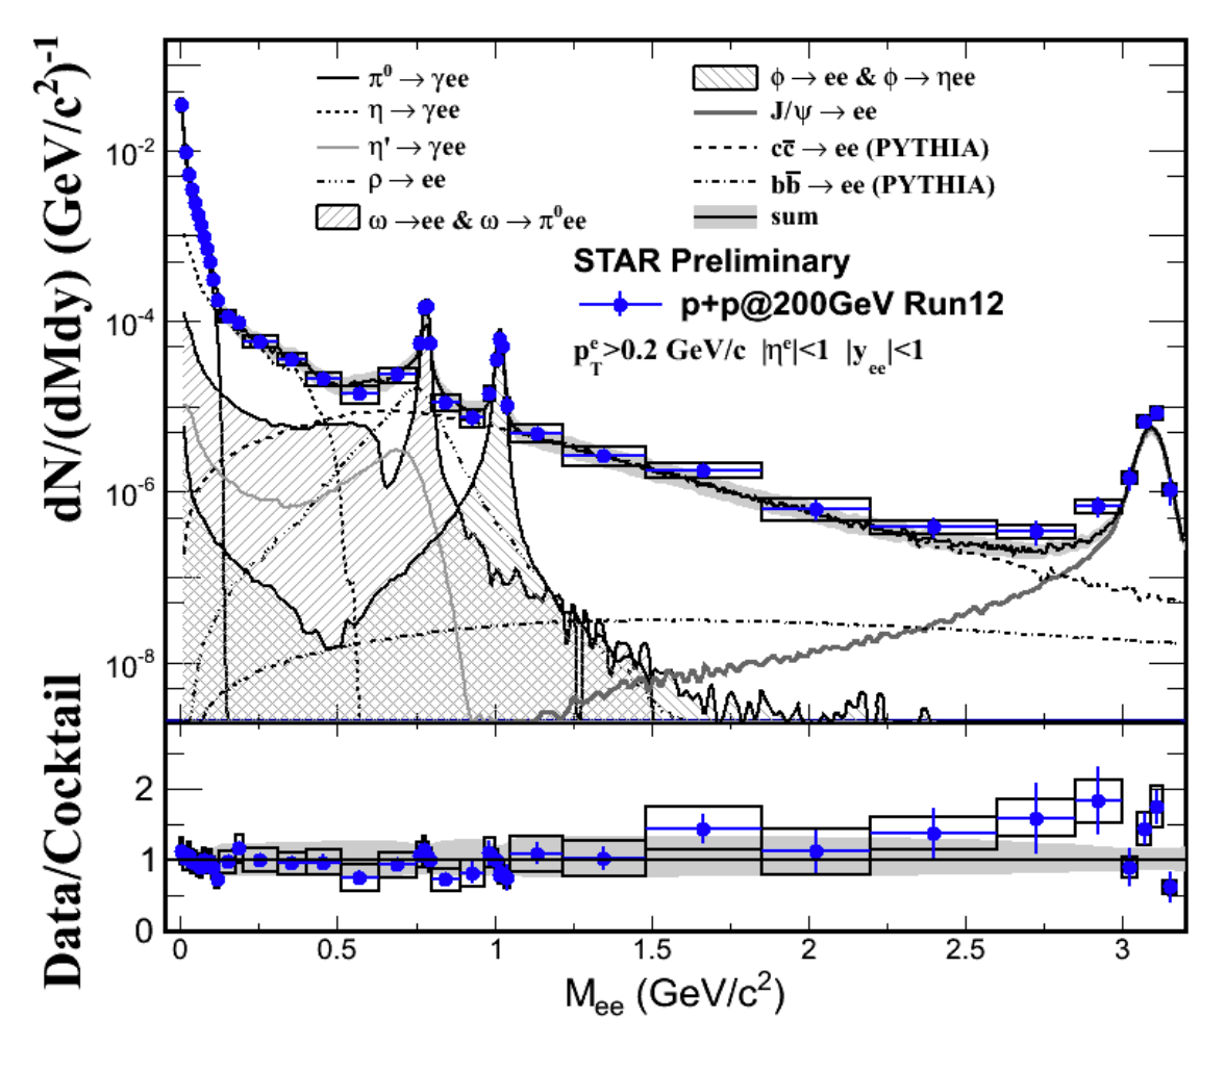
\includegraphics[width=\textwidth,clip]{figures/Chapter1/STARpp.png}
        \caption{}
        \label{fig:STARpp}
    \end{subfigure}
    \hfill
    \begin{subfigure}[b]{0.43\textwidth}
        \centering
        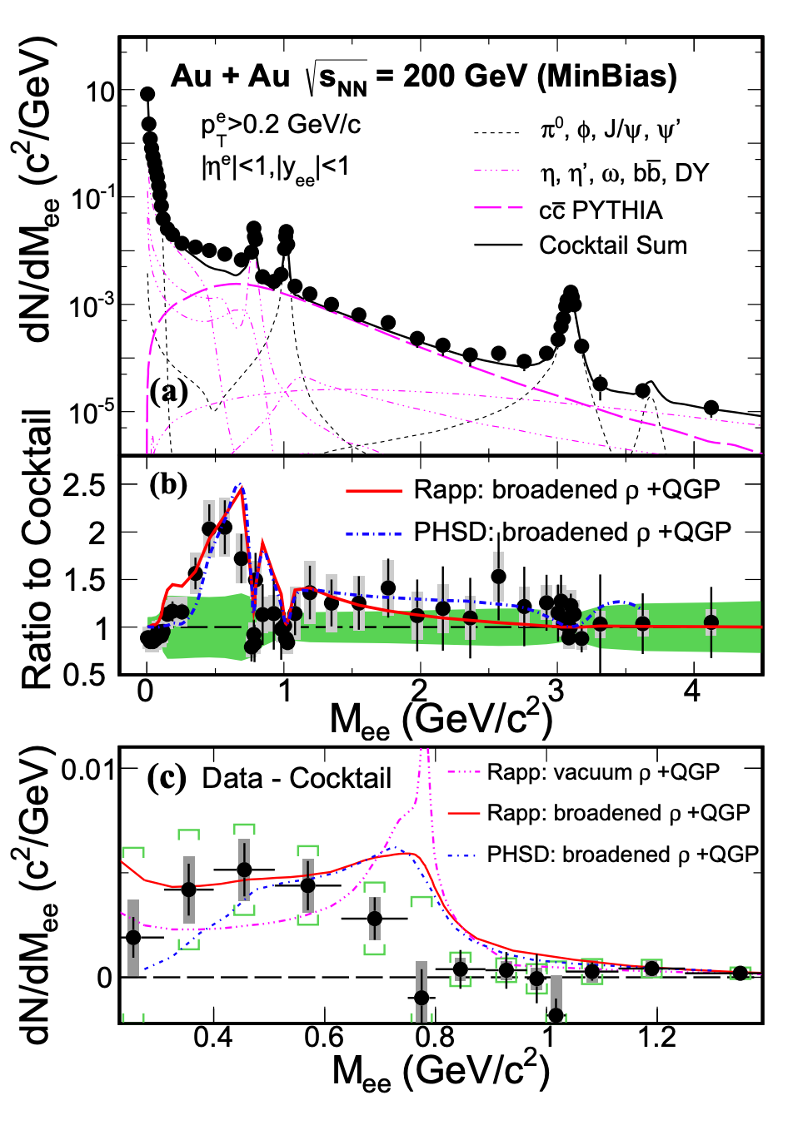
\includegraphics[width=\textwidth,clip]{figures/Chapter1/STARAuAu200.png}
        \caption{}
        \label{fig:STARAuAu}
    \end{subfigure}
    \caption[STAR实验 \sNN = 200 GeV 质子-质子和金-金对撞中的双电子谱测量结果]{STAR实验在其接收度下的 \sNN = 200 GeV 质子-质子和金-金对撞中的双电子谱测量结果。左图为质子-质子对撞中的双电子谱测量结果。测量结果与强子衰变模拟的结果进行比较,强子衰变模拟的不同双电子源在图中已经标出。右图的(a)部分为\sNN = 200 金-金对撞中0-80\%中心度下的双电子谱和强子衰变模拟的结果。(b)部分为数据和强子衰变模拟的比值,(c)部分为额外产额(data-cocktail),并且和几种不同的理论模型相比较}
       \label{fig:STARDiElectron}
\end{figure}

随着能量扫描(Beam Energy Scan)的进行,STAR在多个能量下对金-金对撞中的双电子谱进行了系统的测量。图展示了STAR在 \egyfive 金-金对撞中 0-80\%中心度下的双电子谱。在多个能量下STAR都观测到了在 $\rho$ 质量区间的产额增强。同时STAR在 \sNN = 19.6 GeV的金-金对撞中经过$dN_{ch}/d\eta$归一化和STAR接收度修正后额外产额和 NA60 \sNN = 17.3 GeV 铟-铟对撞下的额外产额可以很好的符合,结果见图 \ref{fig:STAR19p6}。理论模型也可以很好的描述\sNN = 19.6 GeV下双轻子额外产额。

\begin{figure}[htb]
    \begin{center}
    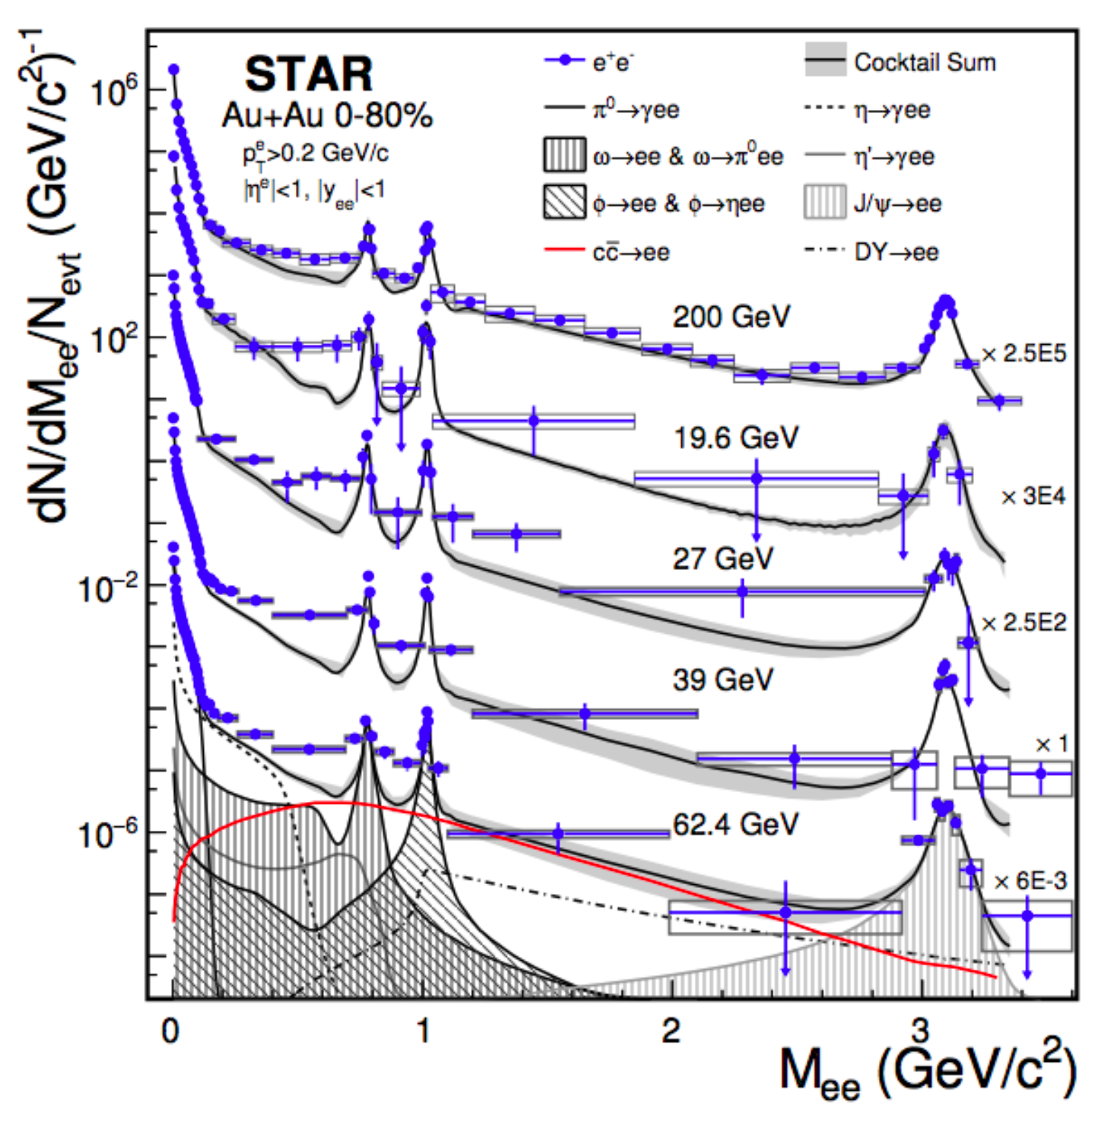
\includegraphics[width=0.6\textwidth,clip]{figures/Chapter1/STARBES.png}
    \end{center}
    \caption[STAR实验 \egyfive 下的双轻子谱]{STAR实验 \sNN = 19.6,27,39,62.4和200GeV下的双轻子谱。系统误差和统计误差分别用方框和竖线列出。图中仅展示了 \sNN = 62.4 GeV的强子衰变模拟结果,其余结果均与各自能量下的强子衰变模拟结果进行比较。}
    \label{fig:STARBES}
\end{figure}

\begin{figure}[htb]
    \begin{center}
    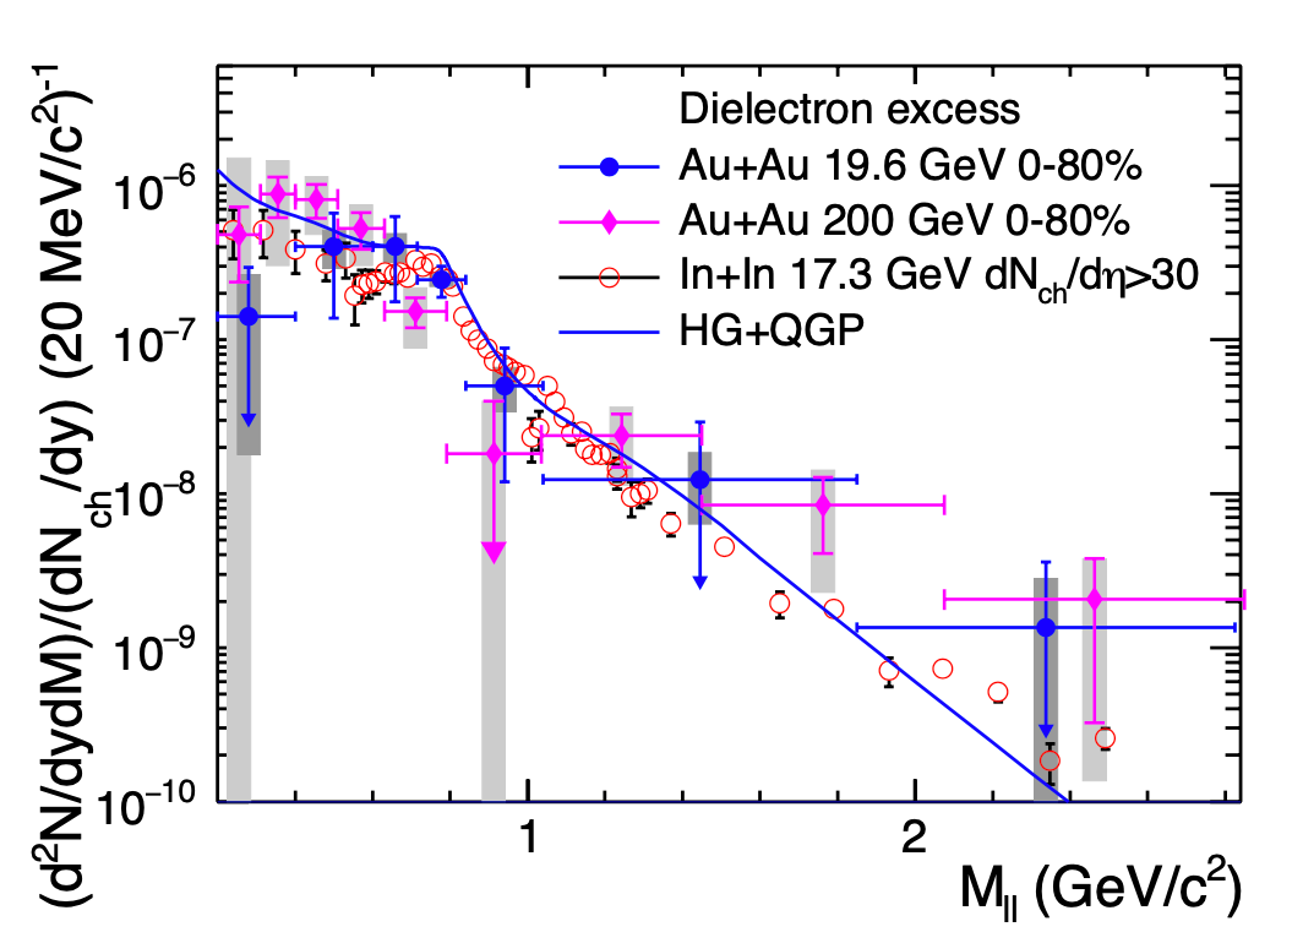
\includegraphics[width=0.6\textwidth,clip]{figures/Chapter1/STAR19p6.png}
    \end{center}
    \caption[STAR实验 \sNN = 19.6和200 GeV 的双轻子谱额外产额和NA60的额外产额比较]{STAR实验 \sNN = 19.6和200 GeV 的双轻子谱额外产额在经过中间快度区间的带电粒子多重数归一化和STAR接收度修正后和NA60的额外产额比较。蓝色实线为包含强子气(Hadron Gas)中broaden $\rho$ 和 QGP热辐射贡献的模型计算结果。 }
    \label{fig:STAR19p6}
\end{figure}

在 \sNN = 200GeV 的情况下,虽然有很高的统计但是随着对撞能量的增加,来源于重味夸克的双轻子在中等质量区间所占的产额比例逐渐增加,导致STAR在\sNN = 200GeV 双轻子测量中难以去抽取来自夸克胶子等离子体的热辐射产额。而在 \sNN = 19.6, 27, 39, 62.4 GeV 几个对撞能量下,虽然重味夸克的截面相比于\sNN = 200GeV 有所降低,但受限于统计也无法在中等质量区间进行热辐射产额的抽取。2017年STAR采集了大约12亿个\sNN = 54.4 GeV的金-金对撞事例。使得STAR有足够的统计在较低的对撞能量下尝试抽取来自于热辐射的双轻子产额。